\documentclass[a4paper,10pt,twocolumn,oneside]{article}
\setlength{\columnsep}{10pt}                                                              %兩欄模式的間距
\setlength{\columnseprule}{0pt}                                                                %兩欄模式間格線粗細

\usepackage{amsthm}								%定義，例題
\usepackage{amssymb}
%\usepackage[margin=2cm]{geometry}
\usepackage{fontspec}								%設定字體
\usepackage{color}
\usepackage[x11names]{xcolor}
\usepackage{listings}								%顯示code用的
%\usepackage[Glenn]{fncychap}						%排版，頁面模板
\usepackage{fancyhdr}								%設定頁首頁尾
\usepackage{graphicx}								% 圖形相關：用於插入與處理圖片 (graphics)
\usepackage{enumerate}
\usepackage{titlesec}
\usepackage{amsmath}
\usepackage{tikz}
\usepackage{xpatch}
\usepackage[CheckSingle, CJKmath]{xeCJK}
% \usepackage{CJKulem}
%\usepackage[T1]{fontenc}
\titlespacing{\section}{0cm}{0cm}{0cm}
\titlespacing{\subsection}{0cm}{0cm}{0cm}
\usepackage{amsmath, courier, listings, fancyhdr, graphicx}
\topmargin=0pt
\headsep=5pt
\textheight=780pt
\footskip=0pt
\voffset=-40pt
\textwidth=545pt
\marginparsep=0pt
\marginparwidth=0pt
\marginparpush=0pt
\oddsidemargin=0pt
\evensidemargin=0pt
\hoffset=-42pt

%\renewcommand\listfigurename{圖目錄}
%\renewcommand\listtablename{表目錄} 

%%%%%%%%%%%%%%%%%%%%%%%%%%%%%

\setmainfont [				%主要字型
    Path = .fonts/ttf/,
    UprightFont = *-Regular,
    BoldFont = *-Bold,
    ItalicFont = *-Italic
  ] {Consolas}

\setmonofont [        
    Path = .fonts/ttf/,
    UprightFont = *-Regular
  ] {Monaco}

% \setmainfont{TeX Gyre Termes}
% \setmainfont{Consolas}				%主要字型
% \setmonofont{Monaco}				%主要字型
\setCJKmainfont{PingFang TC}

% \setCJKmainfont{Consolas}			%中文字型
% \setmainfont{sourcecodepro}
\XeTeXlinebreaklocale "zh"						%中文自動換行
\XeTeXlinebreakskip = 0pt plus 1pt				%設定段落之間的距離
\setcounter{secnumdepth}{3}						%目錄顯示第三層

%%%%%%%%%%%%%%%%%%%%%%%%%%%%%
\makeatletter
\lst@CCPutMacro\lst@ProcessOther {"2D}{\lst@ttfamily{-{}}{-{}}}
\@empty\z@\@empty
\makeatother
\lstset{											% Code顯示
language=Python,										% 設定程式碼區塊語言 (例如 Python, C++, Java)
basicstyle=\footnotesize\ttfamily, 						% 程式碼字型與大小
%numbers=left,										% 是否顯示行號 (註解來停用)
numberstyle=\footnotesize,						% 行號字型大小
stepnumber=1,										% 行號步進 (1 表示每行都編號)
numbersep=5pt,										% 行號與程式碼之間的間距
backgroundcolor=\color{white},					% 程式碼區塊背景色 (預設為白色)
showspaces=false,									% 是否以特定符號顯示空格 (false 表示不顯示)
showstringspaces=false,							% 字串內空格是否顯示 (false 表示不顯示)
showtabs=false,									% 是否顯示 tab 字元
frame=false,											% 是否為程式碼區塊加外框
tabsize=2,											% Tab 的空格寬度 (預設 2)
captionpos=b,										% 標題 (caption) 位置 (b 底部)
breaklines=true,									% 是否自動換行
breakatwhitespace=false,							% 是否只在空白處換行
escapeinside={\%*}{*)},							% 在程式碼中插入 LaTeX 命令或註解的分隔符
morekeywords={*},									% 額外要強調的關鍵字列表
keywordstyle=\bfseries\color{Blue1},
commentstyle=\itshape\color{Red4},
stringstyle=\itshape\color{Green4},
}

%%%%%%%%%%%%%%%%%%%%%%%%%%%%%

\begin{document}
\pagestyle{fancy}
\fancyfoot{}
%\fancyfoot[R]{\includegraphics[width=20pt]{ironwood.jpg}}
\fancyhead[L]{print("世界で一番のPython CodeBook")}
\fancyhead[R]{\thepage}
\renewcommand{\headrulewidth}{0.4pt}
\renewcommand{\contentsname}{Contents} 

\scriptsize
\tableofcontents
%%%%%%%%%%%%%%%%%%%%%%%%%%%%%

% \newpage
\section{Basic}
\subsection{標準輸入}
\lstinputlisting{basic/input.py}
\subsection{標準輸出}
\lstinputlisting{basic/output.py}
\subsection{運算子}
\lstinputlisting{basic/operators.py}
\subsection{型別檢查}
\lstinputlisting{basic/type.py}
\subsection{其他}
\lstinputlisting{basic/other.py}

\section{Data Structure}
\subsection{列表 List}
請注意 Python List 的 Index：
alphabet = ['a', 'b', 'c']  
- POS\_Index: 0,    1,  2
- NEG\_Index: -3,  -2, -1
\lstinputlisting{ds/list.py}
\subsection{元組 Tuple}
請注意 Python 的 tuple 是不可變的 (immutable)。
但 tuple 的內容可以包含可變更的物件 (例如 list)。
請注意 Python Tuple 的 Index：
alphabet = ('a', 'b', 'c')  
- POS\_Index: 0,    1,  2
- NEG\_Index: -3,  -2, -1
\lstinputlisting{ds/tuple.py}
\subsection{集合 Set}
請注意 Python 的 Set 是無序的 (unordered)。
set 的內容也不可以包含可變更的物件 (例如 list)。
\lstinputlisting{ds/set.py}
\subsection{字典 Dict}
\lstinputlisting{ds/dict.py}
\subsection{字串 String}
請注意 Python 的 String 其實是不可變的 (immutable)。
任何對 string 的修改本質上其實是創建一個新的字串物件
請注意 Python String 的 Index：
alphabet = "a   b  c" (忽略空格)
- POS\_Index:0   1  2
- NEG\_Index:-3 -2 -1
\lstinputlisting{ds/string.py}
\subsection{堆疊 Stack}
\lstinputlisting{ds/stack.py}
\subsection{佇列 Queue}
\lstinputlisting{ds/queue.py}
\subsection{鏈結串列 Link List}
\lstinputlisting{ds/linklist.py}
\subsection{二元樹 Binary Tree}
\lstinputlisting{ds/btree.py}

\section{函式 Function}
\subsection{你該知道的事 Things You Should Know}
預設參數 (default arguments)，當呼叫函式時沒有提供對應的參數值，則會使用預設參數值。
但預設參數只會被評估一次，所以千萬不要放可變物件 (mutable objects) 當作預設參數值，否則會發生鬼故事。
預設參數必須放在非預設參數的後面，否則會發生語法錯誤。
\lstinputlisting{function/defaultArg.py}

Python 的變數優先級：
Local (區域) -> Enclosing (封閉) -> Global (全域) -> Built-in (內建) 。
- global : 在函式內修改全域變數。
- nonlocal : 在巢狀函式中修改外層（非全域）變數。

用來判斷目前的模組是否是被直接執行，而不是被其他模組匯入 (import)：
\begin{verbatim}
if __name__ == "__main__":
\end{verbatim}
\subsection{位置參數與關鍵字參數 Positional and Keyword Arguments}
\lstinputlisting{function/pos_and_key.py}

\subsection{可變長度參數 Variable-length Arguments}
*args: 將傳入的多個「位置參數」打包成一個 tuple 傳給 Function。
**kwargs: 將傳入的多個「關鍵字參數」打包成一個 dict 傳給 Function。
\lstinputlisting{function/varArg.py}

\subsection{高階函式 Higher-Order Functions}
\lstinputlisting{function/higherOrderFunction.py}

\subsection{閉包 Closure}
\lstinputlisting{function/closure.py}

\subsection{Lambda 函式 Lambda Functions}
\lstinputlisting{function/lambda.py}

\subsection{內建高階函式 Built-in Higher-Order Functions}
\begin{itemize}
    \item map(function, iterable): 將一個函式應用到一個（或多個）可迭代物件 (iterable) 的每一個元素上，並回傳一個迭代器。
    \item filter(function, iterable): 根據一個函式（該函式回傳 True 或 False）來過濾一個可迭代物件，只保留使 function 回傳 True 的元素，並回傳一個 filter 物件 (可轉換成 list)。
    \item reduce(function, iterable): 將一個可迭代物件中的元素，使用一個函式（該函式接受兩個參數）進行「累加」計算，最終回傳一個單一的值。
\end{itemize}
\lstinputlisting{function/builtInHOF.py}

\subsection{裝飾器 Decorators}
裝飾器（Decorator）是一種設計模式，允許在不改變函式原始碼的情況下，為函式添加額外的功能。
裝飾器本質上是高階函式（Higher-Order Function），接受一個函式作為參數，並回傳一個新的函式。
可以想像成......
\begin{itemize}
    \item 你的函式：你寫好了一個函式，這是「禮物」。例如，一個計算階乘的函式。
    \item 裝飾器：這是一張「包裝紙」。這張包裝紙本身也是一個函式，它定義了「在打開禮物前要做的事」和「在打開禮物後要做的事」。
    \item @ 符號：這個符號就是「包裝動作」。當你把 @XXXXXXX 放在你的函式上面時，你就等於是說：「嘿，Python，請用這張『XXXXXXX包裝紙』把我的『禮物函式』包起來。」
    \item 最終，當我們呼叫被裝飾過的函式時，實際上執行的是 wrapper 函式，而不是原始的 function (my\_decorator 或 timing\_decorator)。
\end{itemize}
\lstinputlisting{function/decorator1.py}
\lstinputlisting{function/decorator2.py}

\subsection{迭代器 Iterators}
迭代器是一種物件，它實現了迭代協定（即 \_\_iter\_\_() 和 \_\_next\_\_() 方法），可以用來遍歷容器（如 list、tuple、dict 等）的元素。
Iterable (可迭代物件)：像是 list，你可以從它身上取得迭代器。
Iterator (迭代器)：是 iter() 函式回傳的物件，它會記住當前位置，並可用 next() 取出下一個值。
\lstinputlisting{function/iterator1.py}
Python 中有很多內建的物件都是可迭代的，甚至本身就是迭代器。
\lstinputlisting{function/iterator2.py}

\subsection{產生器 Generators}
產生器（Generator）是一種特殊類型的迭代器，用於在需要時動態生成值，而不是一次性將所有值存儲在記憶體中。
產生器與 return 最本質的差別如下：
\begin{itemize}
    \item return：像一張「單程車票」。當函式執行到 return 時，函式會結束並回傳一個值，之後無法再從該函式繼續執行。
    \item yield：像一個「遊戲存檔點」。當函式執行到 yield 時，函式會暫停並回傳一個值，但保留其狀態，儲存它所有的狀態（記住 a, b, count 這些變數現在的值），以便下次從暫停的地方繼續執行。當你要求下一個值時（呼叫 next()），函式會從上次凍結的地方「解除暫停」，繼續執行，直到遇到下一個 yield 。
\end{itemize}
\lstinputlisting{function/fibGenerator.py}


\section{File Handling}
\subsection{基本檔案操作 Basic File Operations}
檔案開啟的模式可以分成：
\begin{itemize}
    \item r: 唯讀 (預設)
    \item w: 寫 (覆蓋原有檔案)
    \item a: 附加 (在檔案末尾新增內容)
    \item x: 建立新檔案 (檔案已存在會失敗)
    \item b: 二進位 (與其他模式結合使用，如 rb, wb)
    \item t: 文字模式 (預設，與其他模式結合使用，如 rt, wt)
    \item +: 讀寫模式 (與其他模式結合使用，如 r+, w+)
\end{itemize}
\lstinputlisting{ocfile/openf.py}

\section{Exception Handling}
\subsection{基本例外處理 Basic Exception Handling}
常見的內建例外類型：
\begin{itemize}
    \item ValueError：傳入無效的值（例如 int("abc")）。
    \item TypeError：對不相容的型別進行操作（例如 "5" + 5）。
    \item IndexError：使用了無效的索引值。
    \item KeyError：使用了字典中不存在的鍵。
    \item ZeroDivisionError：除以零 。
    \item FileNotFoundError：試圖開啟不存在的檔案 。
    \item AttributeError：試圖存取物件沒有的屬性或方法。
    \item EOFError：檔案讀取到結尾。
\end{itemize}
\lstinputlisting{exception/exceptionBasic.py}
\subsection{else 和 finally 子句 else and finally Clauses}
\begin{itemize}
    \item `else` 子句：只有在 try 區塊中「沒有」發生任何例外時，else 區塊的程式碼才會被執行 。
    \item `finally` 子句：無論是否發生例外（無論是成功、發生錯誤被捕捉、或發生錯誤未被捕捉），finally 區塊的程式碼「永遠」會被執行 。
\end{itemize}
\lstinputlisting{exception/else-finally.py}
\subsection{自訂例外 Custom Exceptions}
可以透過繼承內建的 Exception 類別來建立自訂的例外類型。
\lstinputlisting{exception/customError.py}
\subsection{斷言 Assertions}
assert 用來檢查一個條件是否為 True。如果條件為 False，assert 會引發 AssertionError 例外。
assert 通常用被拿來當作程式碼中的內部檢查點 (internal checkpoints)，以確保程式在執行過程中符合預期的狀態
assert 的錯誤用法：
\begin{itemize}
    \item 驗證使用者輸入
    \item 驗證外部資料（如檢查檔案是否存在）
    \item 取代正常的錯誤處理邏輯
    \item 在生產環境中依賴 assert 來維護程式邏輯
\end{itemize}
\lstinputlisting{exception/assertSample.py}

\section{Object-Oriented}
\subsection{建立類別 Class Declaration}
\lstinputlisting{oop/oopBasic.py}
\subsection{類別的方法 Class Methods}
\lstinputlisting{oop/oopMethod.py}
\subsection{建構子跟解構子 Constructor and Destructor}
\lstinputlisting{oop/constr_and_deconstr.py}
\subsection{封裝 Encapsulation}
\lstinputlisting{oop/encapsulation.py}
\subsection{封裝屬性 Encapsulation with Property}
@property 裝飾器 (Decorator) 可以把方法轉換成屬性。
比如說，`obj.x` 像是在讀某個值，但實際上是呼叫 `obj.x()`(getter) 方法來取得值。
在比如說，`obj.x = value` 像是在設定某個值，但實際上是呼叫 `obj.x(value)`(setter) 方法來設定值。
\lstinputlisting{oop/property.py}
\subsection{繼承 Inheritance}
基本繼承：
\lstinputlisting{oop/inheritance.py}
多重繼承：
\lstinputlisting{oop/multiInheritance.py}
\subsection{多型 Polymorphism}
\lstinputlisting{oop/polymorphism.py}

\section{Algorithm}
\subsection{矩陣操作 Matrix Operations}
\lstinputlisting{algo/matrix.py}
\subsection{Sort: Bubble Sort}
\lstinputlisting{algo/bubbleSort.py}
\subsection{Sort: Selection Sort}
\lstinputlisting{algo/selectionSort.py}
\subsection{Sort: Insertion Sort}
\lstinputlisting{algo/insertionSort.py}
\subsection{Sort: Quick Sort}
\lstinputlisting{algo/qsort.py}
\subsection{Sort: Quick Sort(In Place)}
\lstinputlisting{algo/qsortip.py}
\subsection{Sort: Merge Sort}
\lstinputlisting{algo/mgsort.py}
\subsection{Search: Binary Search}
\lstinputlisting{algo/binarySearch.py}
\subsection{String: KMP}
\lstinputlisting{algo/kmp.py}

\iffalse
\section{Lab and Homework}
\subsection{week2}
LAB: Digital-Ladder-Matrix
\lstinputlisting{lab-and-hw/week2/lab2-1_Digital-Ladder-Matrix.py}
LAB: Sequence-Sorting
\lstinputlisting{lab-and-hw/week2/lab2-2_Sequence-Sorting.py}
HW: Triangle
\lstinputlisting{lab-and-hw/week2/hw2-1_Triangle.py}
HW: Median
\lstinputlisting{lab-and-hw/week2/hw2-2_Median.py}

\subsection{week3}
LAB: Common-Friends-Finder
\lstinputlisting{lab-and-hw/week3/lab3-1_Common-Friends-Finder.py}
LAB: Train-Station-Stack-Problem
\lstinputlisting{lab-and-hw/week3/lab3-2_Train-Station-Stack-Problem.py}
HW: Most-Frequent-Character
\lstinputlisting{lab-and-hw/week3/hw3-1_Most-Frequent-Character.py}
HW: Binary-Tree-Height
\lstinputlisting{lab-and-hw/week3/hw3-2_Binary-Tree-Height.py}

\subsection{week6}
LAB: Primary-Arithmetic
\lstinputlisting{lab-and-hw/week6/lab4-1_Primary-Arithmetic.py}
LAB: Cola
\lstinputlisting{lab-and-hw/week6/lab4-2_Cola.py}
HW: GCD
\lstinputlisting{lab-and-hw/week6/hw4-1_GCD.py}
HW: Palindromes
\lstinputlisting{lab-and-hw/week6/hw4-2_Palindromes.py}

\subsection{week7}
LAB: Rewriting-The-Three-Little-Pigs
\lstinputlisting{lab-and-hw/week7/lab5-1_Rewriting-The-Three-Little-Pigs.py}
LAB: Company-Salaries
\lstinputlisting{lab-and-hw/week7/lab5-2_Company-Salaries.py}
HW: Guess-Number
\lstinputlisting{lab-and-hw/week7/hw5-1_Guess-Number.py}
HW: Student-Score-Registration
\lstinputlisting{lab-and-hw/week7/hw5-2_Student-Score-Registration.py}

\subsection{week8}
LAB: BankAccount
\lstinputlisting{lab-and-hw/week8/lab6-1_BankAccount.py}
LAB: Quick-Sort
\lstinputlisting{lab-and-hw/week8/lab6-2_Quick-Sort.py}
HW: Vehicle-Management
\lstinputlisting{lab-and-hw/week8/hw6-1_Vehicle-Management.py}
HW: Matrix-Operation
\lstinputlisting{lab-and-hw/week8/hw6-2_Matrix-Operation.py}
HW: Quick-Sort-In-Place
\lstinputlisting{lab-and-hw/week8/hw6-3_Quick-Sort-In-Place.py}
HW: Knuth-Morris-Pratt
\lstinputlisting{lab-and-hw/week8/hw6-4_Knuth-Morris-Pratt.py}

\subsection{week9}
LAB: Text-Frequency-Analyzer
\lstinputlisting{lab-and-hw/week9/lab7_1_func.py}
\lstinputlisting{lab-and-hw/week9/lab7_1_Text-Frequency-Analyzer.py}
LAB: Matrix-Operation
\lstinputlisting{lab-and-hw/week9/lab7-2_Matrix-Operation.py}
HW: Range-Query-Analyzer
\lstinputlisting{lab-and-hw/week9/hw7-1_Range-Query-Analyzer.py}
HW: Nested-String-Expander
\lstinputlisting{lab-and-hw/week9/hw7-2_Nested-String-Expander.py}

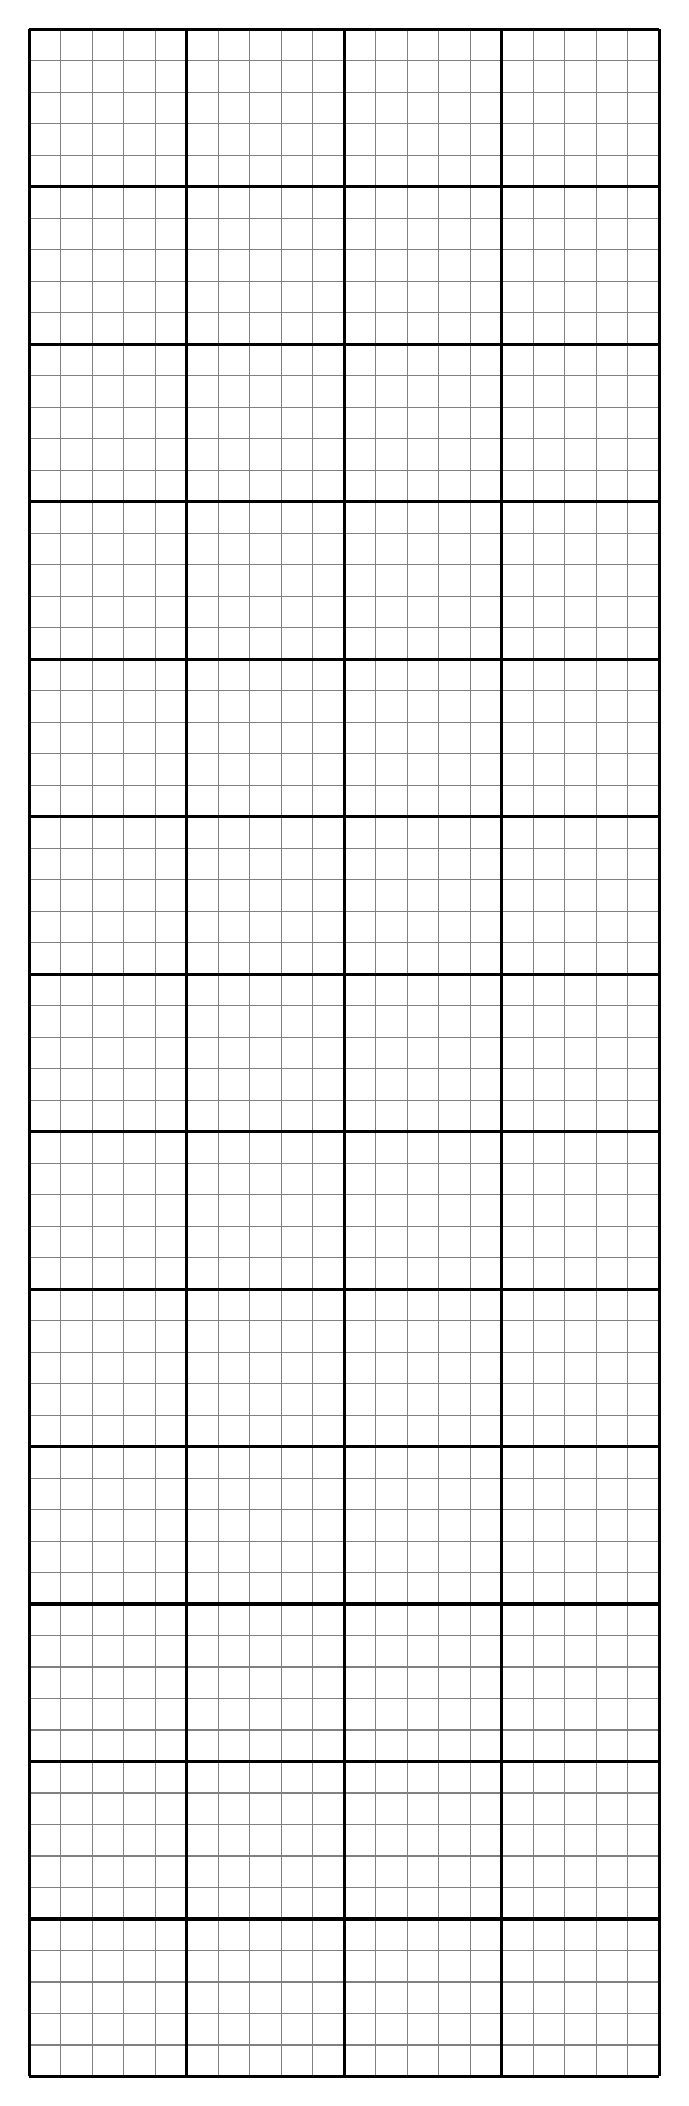
\begin{tikzpicture}[every node/.style={minimum size=1cm-\pgflinewidth, outer sep=10pt}, scale=2]
    \draw[step=0.2cm,color=gray] (0,0) grid (4,13);
    \draw[step=1cm,color=black,line width=0.4mm] (0,0) grid (4,13);
\end{tikzpicture}
\fi

\end{document}